%%%%%%%%%%%%%%%%%%%%%%%%%%%%%%%%%%%%%%%%%
%%%%%%%%%% Content starts here %%%%%%%%%%
%%%%%%%%%%%%%%%%%%%%%%%%%%%%%%%%%%%%%%%%%

\begin{frame}{Агенда}
	\begin{itemize}
	  \item Вовед
	  \item Мотивација
	  \item Хипотеза
	  \item Дизајн и имплементација
	  \item Идеи за идна работа
	  \item Заклучок
	\end{itemize}
\end{frame}

\begin{frame}{Мотивација}{Програмирање}
    \begin{itemize}
      \item Програмирањето е една од основните практични вештини која што се
      изучува во програмите на информатичките факултети и секундарна вештина на
      многу други технички факултети
      \item Големата побарувачка на пазарот на трудот за програмери е една од
      причините за интересот и популарноста меѓу идните студенти
      \item Резултат се големи групи студенти во воведните курсеви
    \end{itemize}
\end{frame}

\begin{frame}{Мотивација}{10 години}
\begin{itemize}
  \item Но програмирањето не е лесно!
  \item Истражувачите (Bloom (1985), Bryan \& Harter (1899), Hayes (1989),
  Simmon \& Chase (1973)) имаат покажано дека се потребни околу десет години
  да се постигне одредено ниво на експертиза во многу различни области како играње
  шах, компонирање музика, работа со телеграф, сликање, свирење пиано, пливање,
  тенис и многу други.
  \item Програмирањето не е исклучок (Winslow (1996))
  \item Потребно е да се решат голем број основни алгоритамски проблеми
      (повеќе од една третина од времето)
\end{itemize}

\end{frame}

\begin{frame}{Потешкотии при програмирање}
\begin{enumerate}
  \item Инсталација и поставување околина за програмирање 
  \item Користење текстуален едитор за код
  \item Разбирање на проблемот и користење програмски јазик за пишување код
  \item Разбирање на грешките при компајлирање
  \item Дебагирање (откривање грешки)
\end{enumerate}
\end{frame}

\begin{frame}{Хипотеза}{Цел на истражувањето}
\begin{itemize}
  \item Олеснување на учењето програмирање кај почетници со помош на напредна
  веб-базирана околина која овозможува чести и информативни повратни
  информации
  \item Зголемување на мотивираноста и успехот на студентите во воведните
  курсеви
  \item Помош на наставниот кадар во администрација на големите групи со
  студенти
\end{itemize}
\end{frame}

\begin{frame}{Предложена методологија}
    \begin{itemize}
      \item Прашалници и анкети
      \item Обработка на статистиката за користење
      \item Анализа и споредба на резултатите 
      \item Издвојување на контролна група
    \end{itemize}
    Седум принципи на добра практика (Chickering
and Gamson (1987))
    \begin{enumerate}
      \item Контакт помеѓу студентот и факултетот
      \item Соработка меѓу студентите
      \item Активно учење
      \item Навремени одговори
      \item Нагласување на временските ограничувања
      \item Соопштување на високите очекувања
      \item Почитување на различностите во талентот и начините на учење
    \end{enumerate}
\end{frame}

\begin{frame}{Што е Code?}
    \begin{itemize}
      \item \emph{Code} е веб-базиран систем за решавање задачи од
      програмирање во почетни курсеви за програмирање
      \begin{itemize}
        \item Интегриран уредувач за код со поглед на задачата
        \item Интегриран уредувач на задачи и тест примери
        \item Автоматско оценување и генерирање повратни информации (feedback)
        \item Управување со корисници и курсеви (централна автентикација)
        \item Подржува различни програмски јазици (C, C++, Java, Python)
        \item Заштитено извршување (Sandbox)
        \item Детекција на плагијати
      \end{itemize}
    \end{itemize}
\end{frame}

\begin{frame}{Архитектура на системот}
    \begin{figure}
    \centering
      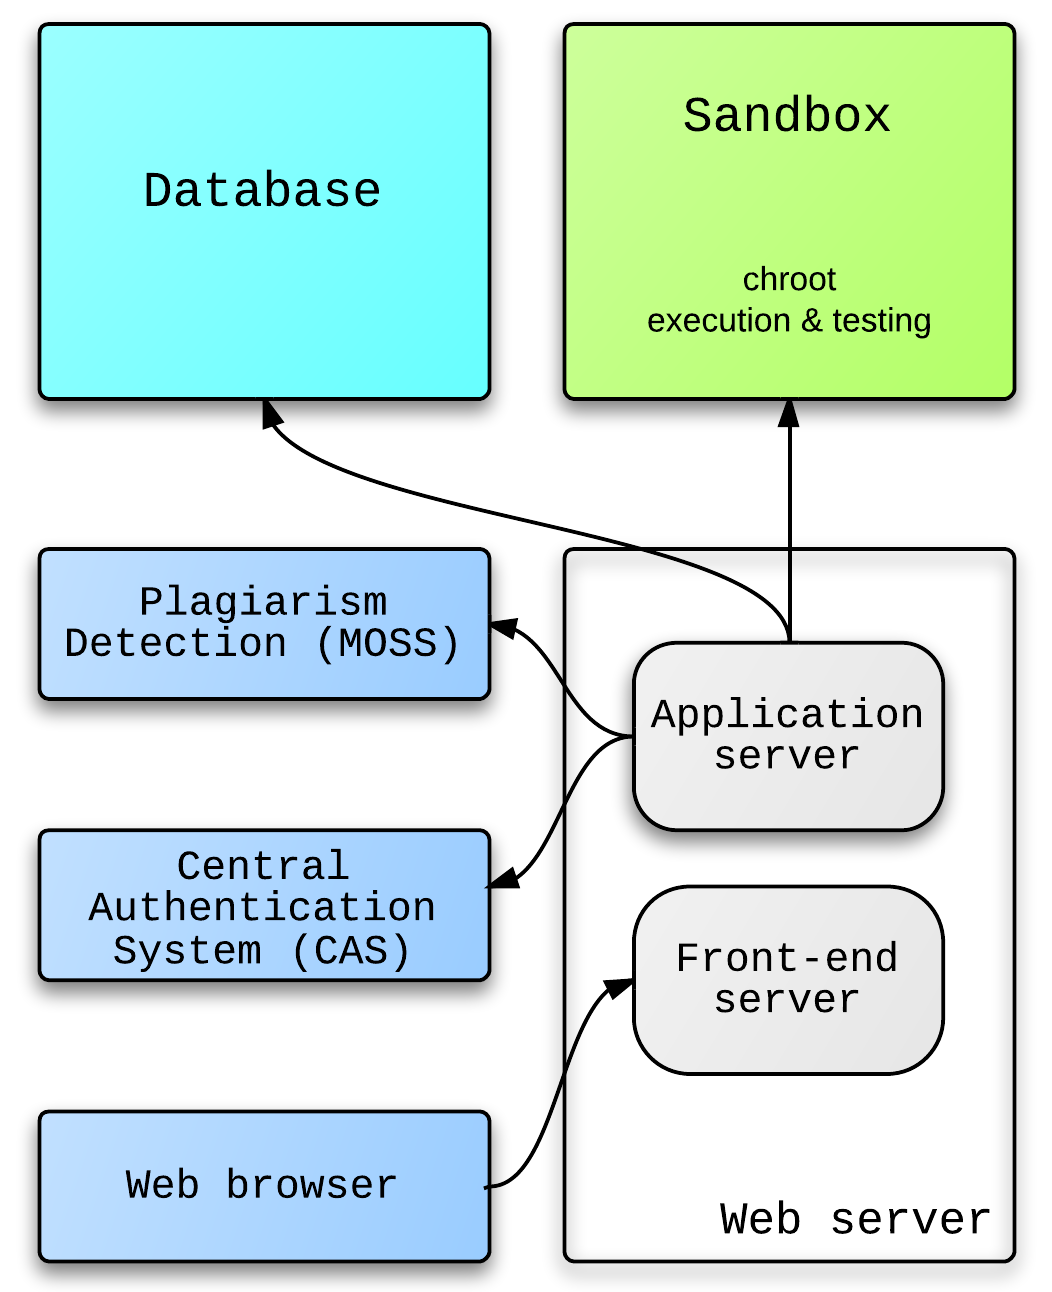
\includegraphics[width=.45\textwidth]{images/architecture-new}        
    \end{figure}
\end{frame}

\begin{frame}{Интегриран поглед на задача}
    \begin{figure}
    \centering
        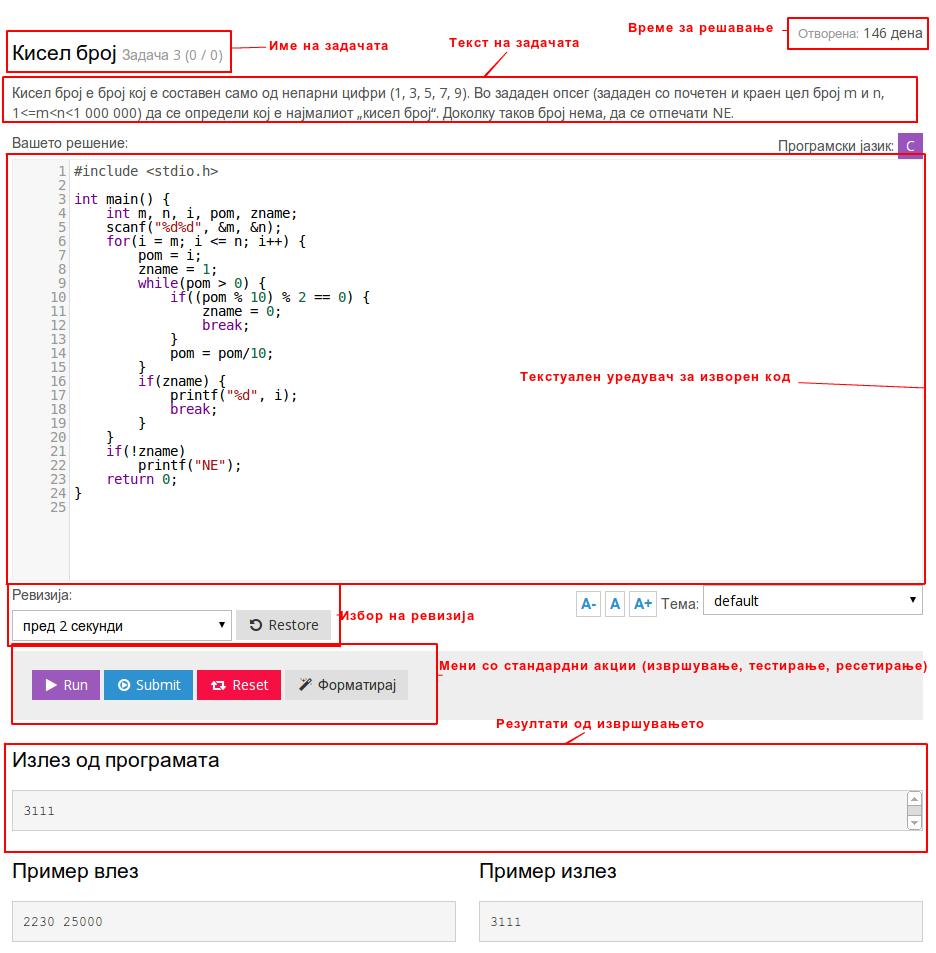
\includegraphics[width=.6\textwidth]{images/integrated_code_view}
        \label{fig:architecture}
    \end{figure}
\end{frame}
  
\begin{frame}{Оценување}{Генерирање повратни информации (feedback)}
\begin{itemize}
  \item Автоматско
  \begin{itemize}
      \item Динамичка анализа
      \item Статичка анализа
  \end{itemize}
  \item Од инструкторите
  \item Помеѓу студентите (peer assesment)
\end{itemize}
\end{frame}

% Define block styles
\tikzstyle{block} = [rectangle, draw, fill=blue!20,
text width=5em, text centered, rounded corners, minimum height=4em]
\tikzstyle{line} = [draw, -latex']

\begin{frame}[fragile]{Динамичка анализа}
    \begin{itemize}
      \item Динамичка анализа или автоматско тестирање е извршување на
      програмата на студентот врз одредено множество на тест податоци
      \item Алгоритамски видови на задачи
      \item Black-box и White-box тестирање
      \item Се користи во системи за натпревари во програмирање
      \item Ја потенцираат важноста во програмирањето да се има решение
      кое работи точно
    \end{itemize}
\end{frame}


\begin{frame}{Статичка анализа}
\begin{itemize}
  \item Процес на анализирање на програмата без да се извршува
  \begin{itemize}
      \item Комплексност
      \item Големина
      \item Разбирливост
      \item Структура на код
  \end{itemize}
  \item Начини на статичка анализа
  \begin{itemize}
      \item Проверка на стилот на програмирање
      \item Детекција на можни грешки
      \item Мерење на карактеристиките со помош на софтверски метрики
      \item Оценување на дизајнот на програмата
      \item Проверка на одредени функционалности
      \end{itemize}
\end{itemize}
\end{frame}


\begin{frame}{Податоци за користење}{Корисници и курсеви}
\begin{itemize}
  \item Корисници
  \begin{itemize}
    \item 2243
  \end{itemize}
  \item Курсеви
\begin{itemize}
  \item Структурно програмирање
  \item Алгоритми и податочни структури
  \item Напредно програмирање
  \item Објектно-ориентирано програмирање
  \item Напредни алгоритми
\end{itemize}
\end{itemize}
\end{frame}

\begin{frame}{Анкета (48 одговори)}{Пристап}
\begin{figure}
    \centering
      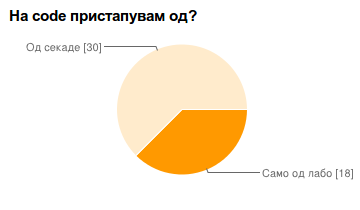
\includegraphics[width=.45\textwidth]{images/responses/pristap}
      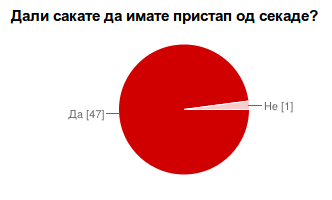
\includegraphics[width=.45\textwidth]{images/responses/od_kade}
    \end{figure}
\end{frame}

\begin{frame}{Анкета (48 одговори)}{Користење и едноставност}
\begin{figure}
    \centering
        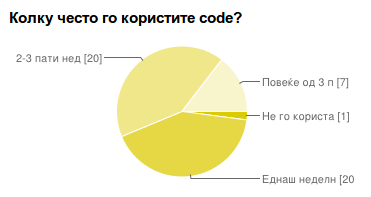
\includegraphics[width=.45\textwidth]{images/responses/usage}
        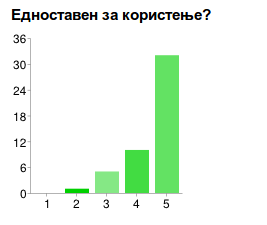
\includegraphics[width=.45\textwidth]{images/responses/simple_to_use}
    \end{figure}
\end{frame}

\begin{frame}{Анкета (48 одговори)}{Приказ и перформанси}
\begin{figure}
    \centering
        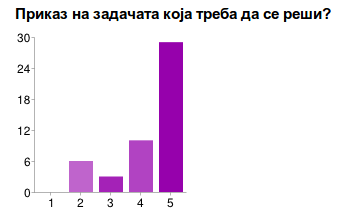
\includegraphics[width=.45\textwidth]{images/responses/prikaz}
        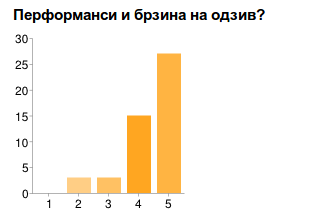
\includegraphics[width=.45\textwidth]{images/responses/performance}
    \end{figure}
\end{frame}

\begin{frame}{Анкета (48 одговори)}{Начин на користење}
\begin{figure}
    \centering
        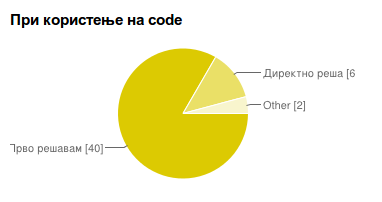
\includegraphics[width=.9\textwidth]{images/responses/ide_vs_code}
    \end{figure}
\end{frame}

\begin{frame}{Анкета (48 одговори)}{Дали Code помага во точно решавање на
задачите}
\begin{figure}
    \centering
        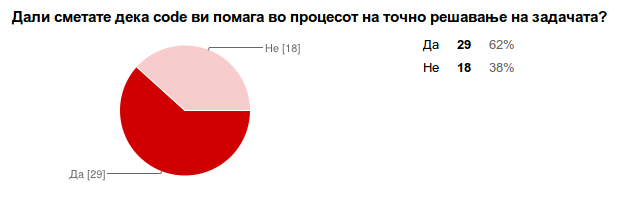
\includegraphics[width=.9\textwidth]{images/responses/is_Code_help}
    \end{figure}
\end{frame}

\begin{frame}{Плагијаризам}
\begin{itemize}
  \item Measure of Software Similarity (MOSS) - A. Aiken
  \item Направена е анализа за плагијaризмот во рамките на два предмети \textbf{Концепти за
развој на софтвер (C)} и \textbf{Напредно програмирање (Java)}
    \item Кај задачите од лабораториски вежби („контролирана средина“)
забележани се бројни плагијати (на некои задачи и преку 30\%)
    \item Кај испитите и колоквиумите не се забележани случаи на плагијати
    \item Постојат и позитивни примери на индивидуални домашни работи
\end{itemize}
\end{frame}

\begin{frame}{Заклучок и понатамошна работа}{Досегашна работа}
    \begin{itemize}
      \item Реализација и имплементација на веб-базирана околина за
      програмирање Code
      \item Преглед и споредба со постеочките околини и алатки за
      автоматско оценување на задачи за програмирање
      \item Истражување на теоријата на учење во контекст на техничките науки со
      посебен аспект на програмирањето како практична вештина
      \item Прв чекор за  приклучок кон светските трендови на приближување
      на образованието кон поголема маса на луѓе (MOOC), со користење на
      најновите технологии
    \end{itemize}
\end{frame}



\begin{frame}{Заклучок и понатамошна работа}{Идеи за понатамошна работа}
\begin{itemize}
  \item Збогатување и подобрување на повратните информации (feedback)
  \item Интеграција со систем за учење
  \item Колаборативно учење
  \item Персонализирано и адаптибилно учење
  \item Следење и визуелизација на извршувањето
  \item Архитектура за скалабилна имплементација во облак
\end{itemize}
\end{frame}

\begin{frame}{Колаборативно учење}{Идеи за понатамошна работа}
\begin{itemize}
  \item Тековните истражувања имаат идентификувани многу бенефити од
  колаборативно учење посебно во воведни прогрмерски курсеви (DeClue, 2003; GILD, 2005; McDowell et al.,
2003; Nagappan et al., 2003; Preston, 2005; Wilson et al., 1993)
\item Покажано е дека и крајните резултати се подобри кога студентите работат
заедно за време на семестарот (McDowell et al., 2002; McDowell et al., 2003; Nagappan et al.,
2003)
\item Синхрони алатки (chat, колаборативен едитор)
\item Асинхрони алатки (форуми, емаил)
\end{itemize}
\end{frame}


\begin{frame}{Прашања}{}
    \begin{center}
    \Large{
    \href{http://code.finki.ukim.mk/}{\textbf{http://code.finki.ukim.mk}}}
    \vfill
    \huge{Ви благодарам на вниманието}
    \vfill    
    \Huge{Прашања?}
    \end{center}
\end{frame}







